\section{Empirical Study}\label{sec:empirical}

This section reports the pre-registered real-data study. The design tests three falsifiable claims fixed before any grid run (\Cref{sec:lps}): (i) the sign of the RevIN--CondNorm test-error gap on each dataset is predicted by the $\lps$ decision rule with $\tau=0.3$; (ii) the magnitude of the gap increases monotonically with $\lps$; and (iii) on Jeju Wind the gap at $h=48$ exceeds the gap at $h=24$, as \Cref{sec:theory} predicts. Claim (i) constitutes the second pre-registered go/no-go gate (Gate~2); claims (ii) and (iii) are auxiliary predictions excluded from the gate verdict. Three additional blocks probe the mechanisms behind the result; their full tables appear in \Cref{app:ext}.

\subsection{Data}

We use eight datasets in two groups. The \emph{exogenously-driven} group consists of series whose level is substantially determined by observable external drivers. \textbf{Jeju Wind} is aggregate wind-power generation on Jeju Island, Korea (hourly, July 2021--December 2023; 21{,}720 observations), paired with archived short-term numerical weather prediction (NWP) forecasts from the Korea Meteorological Administration. Forecasts are \emph{lead-matched} to the forecast origin: for horizons $h\le 24$ we use the forecast band issued at 23:00 two days prior (lead times 26--49\,h), and for $h\le 48$ the band issued three days prior (lead times 50--73\,h). The correlation between generation and forecast wind speed is $0.742$ for the day-ahead band and $0.704$ for the longer-lead band---decaying with lead time, as physically expected.\footnote{A transparency
note on dataset provenance: Jeju Wind was curated by us during this study
(data collection, NWP lead-matching, and quality screening were interleaved
with method development), so it should be read as a \emph{development}
dataset. GEFCom2014 and the standard long-horizon benchmarks are third-party
datasets frozen before this project began, and play a confirmation-style
role. The distinction does not affect the pre-registration guarantee: the
sign predictions for all eight datasets---including Jeju Wind---were derived
from the $\lps$ rule and committed (commit \texttt{cab17c1}) before any grid
run on any dataset was launched.} A single archive gap (25 June--4 July 2023) is handled by segment-aware windowing: no training or evaluation window spans the gap, and no values are interpolated. The remaining three series---\textbf{GEFCom-Wind}, \textbf{GEFCom-Load}, and \textbf{GEFCom-Solar}---come from GEFCom2014 \citep{hong2016gefcom} with their published explanatory variables (NWP wind components, temperature, and NWP solar variables, respectively).

We emphasize the leakage discipline for weather covariates: all NWP inputs are \emph{archived operational forecasts matched by issue lead}, never reanalysis products. Reanalyses assimilate observations from the forecast target period and would leak future information into the covariate path---a subtle but fatal flaw for any claim about exogenous predictability.

The \emph{standard} group comprises the long-term-forecasting benchmarks ETTh1, ETTh2, Electricity, and Weather. Here the only covariates supplied to any method are deterministic calendar harmonics, so conditional normalization can exploit seasonal structure but has no genuinely exogenous level information. This group is where the distribution-shift motivation of instance normalization \citep{kim2022revin} is expected to hold.

\subsection{Design and protocol}

Block~A, the pre-registered grid, crosses five normalization arms \{Raw, RevIN, SAN, FAN, CondNorm\} \citep{kim2022revin,liu2023san,ye2024fan} with four backbones \{RLinear, PatchTST, SegRNN, LightGBM-DMS\} \citep{li2023rlinear,nie2023patchtst,lin2023segrnn,ke2017lightgbm}, horizons $h\in\{24,96,336\}$ ($\{24,48\}$ for Jeju Wind, constrained by NWP lead coverage), and seeds $\{0,\dots,4\}$; LightGBM runs are deterministic. The combinations LightGBM$\times$SAN and LightGBM$\times$FAN are structurally infeasible (these arms are learned, backpropagated modules) and were declared N/A at pre-registration; the RevIN analogue for LightGBM is per-window z-normalization. Block~A comprises 1{,}794 runs.

Capacity is controlled to isolate the normalization effect: for each (dataset, backbone, $h$), the lookback is tuned over $\{96,192,336,720\}$ on \emph{validation} loss of the RevIN arm at seed~0, then frozen for all five arms. Thus arms within a cell differ in normalization only---never in depth, width, or lookback. Splits are chronological and out-of-time; the global z-score is fit on the training segment only; loaders use \texttt{drop\_last=False} \citep{qiu2024tfb}; training uses fixed seeds and deterministic kernels (full settings in \Cref{app:repro}).

Three extension blocks reuse this discipline. Block~A is deliberately information-asymmetric: only CondNorm consults the covariates (through its first-stage regression), while the four endogenous arms see the target alone. Block~B (\emph{covariate-fair}; 1{,}133 runs) removes this asymmetry, giving \emph{every} arm identical past and future covariates as inputs across five covariate-capable backbones, so that any residual CondNorm advantage cannot be attributed to covariate access. Blocks~C and~D (1{,}275 runs; 4{,}202 in total) run the arms on published state-of-the-art architectures---TimeXer and iTransformer \citep{wang2024timexer,liu2024itransformer}---with (C) and without (D) their official covariate paths; their built-in \texttt{use\_norm} (equivalent to our RevIN arm) is removed so that normalization enters \emph{only} through the five external arms. The backbone-by-backbone correspondence between published defaults and our arms is audited in \Cref{tab:audit} (\Cref{app:design}). Because training budgets differ across blocks (e.g., epoch caps of 12 in~A and 15 in~B), we never compare numbers \emph{across} blocks; each block is internally uniform and self-contained.

\subsection{Statistical testing}

Significance marks use Diebold--Mariano tests \citep{diebold1995comparing} on the per-$(\text{backbone},h)$ seed-mean loss differentials, with a Bartlett-kernel HAC variance (bandwidth $h-1$, capped at $n/4$) and the small-sample correction of \citet{harvey1997testing}. Dataset-level marks in \Cref{tab:main} combine the cell-level $p$-values by Fisher's method ($p<0.05$).\footnote{Fisher's method assumes independent $p$-values, whereas the
per-(backbone,\,$h$) cells within a dataset share the same test period and
are positively dependent, making the combination anti-conservative. As a
robustness check we recombined all cells with two dependence-robust rules:
under the harmonic-mean $p$-value \citep{wilson2019hmp}, valid under
arbitrary dependence, and under Simes's procedure, $31$ of the $32$ stars
in \Cref{tab:main} are unchanged. The single exception is RevIN on ETTh2
(only $3$ of $9$ cells individually significant; Fisher $p=0.026$,
harmonic-mean $p=0.077$, Simes $p=0.130$), which should be read as
indicative; the qualitative conclusion for ETTh2 (instance normalization
dominates conditional normalization by a wide margin) does not rest on
this mark.} Complementing pairwise tests, we compute the Model Confidence Set \citep{hansen2011mcs} over the five arms within each (dataset, $h$) cell at $\alpha=0.10$, using the $T_{\max}$ statistic and the stationary bootstrap \citep{politis1994stationary}.

\subsection{Pre-registered results}

\begin{table}[t]
\centering
\caption{Main results by dataset. Columns are grouped into \emph{benchmarks} (deterministic, no learned normalization), \emph{endogenous} level handling (the instance-normalization family, plus global $z$-scoring which handles the level with a single train-fitted constant), and \emph{exogenous} level handling. Panel~(a): test MSE on the train-fitted global $z$-score scale, averaged over backbones, horizons, and seeds (Block~A). Panel~(b): the same forecasts in MASE, i.e.\ test MAE divided by the in-sample seasonal-naive MAE of the same series on the same scale \citep{hyndman2006another}, so values are comparable across datasets and $>1$ means worse than a one-step seasonal-naive benchmark fitted in-sample. \textbf{Bold}: row minimum over all nine columns. $^{*}$: significantly worse than the best \emph{normalization} arm ($p<0.05$; DM test with Harvey correction on per-$(\text{backbone},h)$ seed-mean loss differentials, Fisher-combined across cells); the DM machinery is defined within Block~A, so the four benchmark columns carry no marks. Benchmarks are run on the identical chronological splits, window-admissibility rules and $z$-scale as Block~A at the fixed lookback $L=336$ (\Cref{app:ext}); they are deterministic and therefore have no seed variation.}
\label{tab:main}
\small
\setlength{\tabcolsep}{3.2pt}
\begin{tabular}{lcccccccccc}
\toprule
& \multicolumn{4}{c}{Benchmarks} & \multicolumn{4}{c}{Endogenous level} & Exogenous \\
\cmidrule(lr){2-5}\cmidrule(lr){6-9}\cmidrule(lr){10-10}
Dataset & S.\,naive & Clim. & DynReg & FirstStg & Raw & RevIN & SAN & FAN & CondNorm \\
\midrule
\multicolumn{10}{l}{\emph{(a) Test MSE}} \\[2pt]
\multicolumn{10}{l}{\emph{Exogenously-driven group}} \\
Jeju Wind     & $1.6265$ & $1.0320$ & $\mathbf{0.2850}$ & $0.2938$ & $0.6887^{*}$ & $0.6969^{*}$ & $0.7030^{*}$ & $0.7724^{*}$ & $0.2933$ \\
GEFCom-Wind   & $1.9878$ & $1.2312$ & $0.1710$ & $\mathbf{0.1564}$ & $1.1153^{*}$ & $1.0039^{*}$ & $0.9755^{*}$ & $1.1875^{*}$ & $0.1629$ \\
GEFCom-Load   & $0.6860$ & $1.1900$ & $0.3714$ & $0.1365$ & $0.3592^{*}$ & $0.3432^{*}$ & $0.3330^{*}$ & $0.3678^{*}$ & $\mathbf{0.1066}$ \\
GEFCom-Solar  & $0.3329$ & $0.2029$ & $0.1414$ & $\mathbf{0.0565}$ & $0.1828^{*}$ & $0.1844^{*}$ & $0.2116^{*}$ & $0.1833^{*}$ & $0.0580$ \\
\midrule
\multicolumn{10}{l}{\emph{Standard LTSF group}} \\
ETTh1         & $0.6695$ & $0.8826$ & $0.4792$ & $1.4033$ & $0.3962^{*}$ & $\mathbf{0.3771}$ & $0.3910^{*}$ & $0.4114^{*}$ & $2.2016^{*}$ \\
ETTh2         & $0.5769$ & $3.1284$ & $0.8921$ & $3.3670$ & $0.3868^{*}$ & $0.2900^{*}$ & $\mathbf{0.2869}$ & $0.3253^{*}$ & $6.6044^{*}$ \\
Electricity   & $0.2174$ & $0.3894$ & $0.1986$ & $0.3224$ & $0.1500^{*}$ & $0.1458^{*}$ & $0.1443^{*}$ & $\mathbf{0.1375}$ & $0.1726^{*}$ \\
Weather       & $0.3383$ & $0.6876$ & $0.1808$ & $0.6483$ & $0.1815^{*}$ & $0.1719^{*}$ & $\mathbf{0.1666}$ & $0.1747^{*}$ & $0.7274^{*}$ \\
\midrule
\multicolumn{10}{l}{\emph{(b) MASE}} \\[2pt]
\multicolumn{10}{l}{\emph{Exogenously-driven group}} \\
Jeju Wind     & $1.121$ & $1.030$ & $\mathbf{0.462}$ & $0.477$ & $0.776$ & $0.741$ & $0.761$ & $0.803$ & $0.478$ \\
GEFCom-Wind   & $1.225$ & $0.985$ & $0.350$ & $\mathbf{0.335}$ & $0.921$ & $0.885$ & $0.881$ & $0.950$ & $0.345$ \\
GEFCom-Load   & $1.613$ & $2.310$ & $1.186$ & $0.687$ & $1.155$ & $1.123$ & $1.113$ & $1.166$ & $\mathbf{0.564}$ \\
GEFCom-Solar  & $1.288$ & $1.197$ & $1.253$ & $\mathbf{0.554}$ & $1.220$ & $1.239$ & $1.369$ & $1.212$ & $0.587$ \\
\midrule
\multicolumn{10}{l}{\emph{Standard LTSF group}} \\
ETTh1         & $1.219$ & $1.691$ & $1.114$ & $2.064$ & $1.006$ & $\mathbf{0.950}$ & $0.966$ & $1.024$ & $2.549$ \\
ETTh2         & $1.535$ & $4.254$ & $1.963$ & $4.362$ & $1.288$ & $\mathbf{1.090}$ & $1.092$ & $1.192$ & $5.691$ \\
Electricity   & $1.047$ & $1.605$ & $1.089$ & $1.423$ & $0.947$ & $0.926$ & $0.930$ & $\mathbf{0.881}$ & $0.995$ \\
Weather       & $0.754$ & $1.503$ & $0.633$ & $1.237$ & $0.602$ & $\mathbf{0.532}$ & $0.537$ & $0.566$ & $1.300$ \\
\bottomrule
\end{tabular}
\end{table}

\Cref{tab:main} is the paper's central result, and it is a double dissociation between two \emph{strategies} for handling the level, not a ranking of methods. Read the three covariate-conditioned columns---the first-stage regression used alone, the classical dynamic regression, and \cnm---against the best instance-normalized arm in each row. On the exogenously-driven group they win $11$ of the $12$ comparisons; on the standard group they win $0$ of $12$. Under MASE the counts are $10$ of $12$ and $0$ of $12$. Both exceptions are the same method for the same reason: the ridge \emph{DynReg} loses on GEFCom-Load, whose temperature--load response is strongly nonlinear---the identical failure that costs a ridge first stage two hits in the $\lps$ sensitivity check of \Cref{tab:tau}---and, under MASE only, on GEFCom-Solar. No covariate-conditioned model wins on any standard dataset under either measure.

Three further readings matter. First, the effect is not an artifact of a dimensionless scale: panel~(b) puts every number against the same series' own in-sample seasonal-naive error, and the ordering is unchanged. Second, the benchmark columns discipline the interpretation in both directions---on GEFCom-Load and GEFCom-Solar \emph{every} endogenous arm is worse than an in-sample seasonal-naive benchmark (MASE $1.11$--$1.37$), which is the operationally meaningful statement of what the boundary costs, while on the standard group the endogenous arms sit at MASE $0.53$--$1.09$ and the covariate-conditioned ones at $0.99$--$5.69$. Third, the failure of \cnm{} off its region is severe and we do not soften it: on ETTh2 it reaches MSE $6.6044$ against $0.2869$ for the best arm, because calendar harmonics carry essentially no level information and the first-stage regression injects its own error into the restored level. \Cref{sec:discussion} reports what a shrinkage safeguard does and does not repair.

\paragraph{Gate~2: sign predictions} All eight pre-registered sign predictions were confirmed (criterion: at least 6/8). The realized dataset-mean gaps, $\mse(\text{RevIN})-\mse(\text{CondNorm})$, are: Jeju Wind $+0.4037$, GEFCom-Wind $+0.8410$, GEFCom-Load $+0.2366$, GEFCom-Solar $+0.1264$ (all predicted positive), and ETTh1 $-1.8244$, ETTh2 $-6.3145$, Electricity $-0.0268$, Weather $-0.5555$ (all predicted negative). These predictions, the official $\lps$ specification, and $\tau=0.3$ were committed to version control (commit \texttt{cab17c1}) before any grid run was launched.

What this record does and does not show is worth stating precisely, because the natural summary statistic is misleading here. A binomial reference treating each sign as a coin flip would give $2^{-8}\approx 0.004$, but the eight datasets are not eight independent draws: they fall into two internally correlated regimes, and a reader who grants only that the two \emph{regimes} were called correctly is looking at $p = 0.25$. We therefore do not rest any claim on the aggregate hit rate. The informative content is per-dataset and is robust in the ways that can be checked without new runs: the same eight signs are obtained under MAE and under MASE (\Cref{tab:main}b), so the record is not an artifact of squared error on a dimensionless scale; the margins are large relative to seed dispersion on seven of the eight datasets, Electricity being the exception by construction; and the per-dataset magnitudes in \Cref{tab:main} do not depend on treating the datasets as exchangeable. What the record establishes is that a quantity computable before training assigned each of our eight series to the correct side of the boundary; what it cannot establish, with eight series in two clusters, is a calibrated probability that it will do so on the next one.

\paragraph{Model Confidence Sets} At $\alpha=0.10$, the surviving set in \emph{all eleven} exogenous (dataset, $h$) cells is $\{\text{CondNorm}\}$ alone. On the standard cells the survivors are $\{\text{RevIN}\}$ in all three ETTh1 cells, $\{\text{RevIN},\text{SAN}\}$ in all three ETTh2 cells, $\{\text{FAN}\}$ in all three Electricity cells, and $\{\text{SAN}\}$ in all three Weather cells. Across all 23 cells, survival counts are: Raw 0, RevIN 6, SAN 6, FAN 3, CondNorm 11. One property of this output should temper how it is read: the procedure returns a \emph{singleton} in 20 of the 23 cells. A confidence set that almost always contains exactly one element is reporting an ordering rather than quantifying uncertainty about it, which is what one expects when the bootstrap resamples a single realized test path and the arms have been averaged over backbones and seeds beforehand. We therefore treat the model confidence sets as a compact summary of the within-cell ranking, consistent with the pairwise tests, and not as an independent uncertainty statement; the limitation is the single evaluation origin discussed in \Cref{sec:discussion}, which no post-processing of these runs can repair.

\paragraph{The near-boundary case} Electricity sits closest to the threshold ($\lps=0.283<\tau=0.3$) and was flagged in the pre-registration as the lowest-confidence prediction. It behaved accordingly: its realized gap is the smallest in magnitude ($-0.0268$), roughly five times closer to zero than any other dataset, so the boundary is where the two regimes genuinely meet rather than an artifact of dataset selection. We are careful, though, not to overstate how densely the boundary is sampled. The $\lps$ values are strongly bimodal---$0.74$--$0.89$ for the four energy series and $-0.72$--$0.28$ for the four standard benchmarks---with no dataset in between; the wide all-correct plateau of \Cref{tab:tau} ($\tau\in[0.30,0.70]$) therefore falls entirely in this empty inter-cluster gap and reflects the separation between the two regimes as much as any fine calibration of $\tau$. Electricity is the only dataset that lands near the threshold at all, so the rule is genuinely stress-tested at its boundary in effectively a single case ($n=1$). Establishing that the crossover is \emph{sharp} there---rather than that two well-separated clusters are merely distinguishable---will require datasets of intermediate predictability, which we flag as a target for confirmatory replication.

\subsection{Mechanism: the layer, not the information}\label{sec:parity}

\Cref{tab:main} is deliberately information-asymmetric: only \cnm{} consults the covariates, through its first-stage regression, while the four endogenous arms see the target alone. Taken by itself the table is therefore consistent with the objection that this is ``just feature engineering''---a model that sees tomorrow's weather forecast beats models that do not. The information-parity block (Block~B; 1{,}133 runs) removes the asymmetry by supplying \emph{every} arm with the identical past and future covariates as backbone inputs, across five covariate-capable backbones, on the four exogenously-driven datasets. This is the comparison that carries the paper's mechanism claim, so we report it with uncertainty rather than as point estimates.

The operative quantity is the \emph{isolated cost of the normalization layer under equal information}: the paired difference $\mse(\text{RevIN}+\text{cov}) - \mse(\rawm+\text{cov})$, in which the two arms receive the same inputs, the same backbone, the same capacity and the same budget, and differ only in whether the window statistics are removed and mechanically restored. It is positive on every backbone:

\begin{center}
\small
\begin{tabular}{lccc}
\toprule
Backbone & $\mse(\text{RevIN}+\text{cov}) - \mse(\rawm+\text{cov})$ & 95\% CI & cells $>0$ \\
\midrule
LGBM-Cov      & $+0.0191$ & $[+0.0116,\, +0.0269]$ & 11/11 \\
Linear mixer  & $+0.0205$ & $[+0.0056,\, +0.0368]$ & 8/11 \\
MLP mixer     & $+0.0238$ & $[+0.0119,\, +0.0390]$ & 10/11 \\
SegRNN-Cov    & $+0.0112$ & $[+0.0058,\, +0.0172]$ & 10/11 \\
PatchTST-Cov  & $+0.0038$ & $[-0.0091,\, +0.0167]$ & 7/11 \\
\bottomrule
\end{tabular}
\end{center}

\noindent Intervals are cluster bootstraps over the 11 seed-averaged (dataset, horizon) cells, resampling cells rather than origins so that the serial dependence within a test path is not treated as replication. Four of the five differences exclude zero; \textbf{PatchTST-Cov does not}, and we state that as a null rather than absorbing it into a claim about ``every backbone''---its minimal covariate adapter exposes less level information to the backbone than the other four, so it is the arm in which the layer has least to destroy. The magnitudes deserve equal candour: these are differences of $0.004$ to $0.024$ MSE, one to two orders of magnitude below the $+0.841$ headline gap of \Cref{tab:main}. That contrast is the honest shape of the result. The large number measures what covariate access is worth; the small number measures what the normalization layer costs once access is equalized, and only the small number is attributable to the layer.

Two further observations sharpen the mechanism. First, the \rawm$-$\cnm{} gap shrinks as backbone flexibility grows ($+0.127$ for the linear mixer, $+0.052$ for the MLP mixer, $-0.009$ for LightGBM-Cov, i.e.\ \rawm{} slightly ahead), while the RevIN$-$\rawm{} difference above persists at every capacity. A flexible model given raw inputs can learn the covariate-to-level map for itself, which is why \cnm{} loses its advantage there; no model can recover a level its normalizer has already subtracted, which is why the RevIN penalty does not vanish. This is the reparameterization argument of \citet{toner2024linear} applied to a constrained rather than an unconstrained class. We flag the capacity ordering as an exploratory post-hoc observation confined to the mixer ladder: PatchTST-Cov ($+0.142$) sits outside it and SegRNN-Cov is $-0.004$. Second, this is the same dissociation that \Cref{tab:main} shows at the level of strategies, obtained by a different route---there by comparing methods that condition the level on covariates against methods that do not, here by holding the covariates fixed and toggling only the layer.

\subsection{What \texorpdfstring{$\lps$}{LPS} orders, and what it does not}

\begin{figure}[t]
\centering
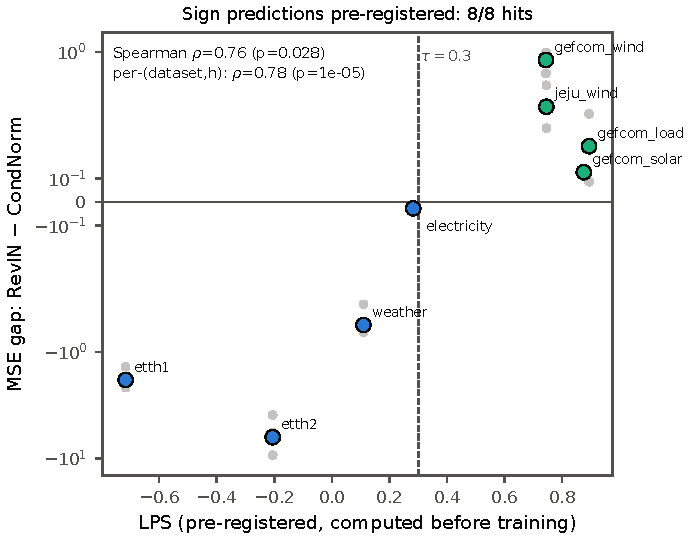
\includegraphics[width=.75\linewidth]{figures/fig3_lps_gap.pdf}
\caption{Realized RevIN$-$CondNorm test-MSE gap versus pre-registered $\lps$, one point per (dataset,\,$h$) cell, coloured by regime. The vertical line marks $\tau=0.3$. The pooled rank association ($\rho=0.783$, $n=23$) is a \emph{between}-regime effect: within the exogenously-driven regime the association reverses ($\rho=-0.750$, $n=11$), so the figure should be read as a separation of two clusters, not as a dose--response curve.}
\label{fig:lpsgap}
\end{figure}

Beyond sign accuracy, the pre-registration recorded an auxiliary prediction (excluded from the gate) that the gap \emph{magnitude} increases with $\lps$. \textbf{We report this prediction as not supported.} Pooled over all 23 (dataset, $h$) cells the rank association is positive and large, $\rho=0.783$; but decomposing it by regime shows that it is entirely a between-cluster effect. Within the exogenously-driven regime the association \emph{reverses}: $\rho=-0.750$ on its 11 cells, and the two datasets with the highest $\lps$ (GEFCom-Load $0.894$ and GEFCom-Solar $0.875$) have the two \emph{smallest} dataset-mean gaps ($+0.237$ and $+0.126$), while the two lowest-$\lps$ exogenous datasets have the largest ($+0.841$ and $+0.404$). Within the standard regime the association is positive ($\rho=+0.777$ on 12 cells). A pooled coefficient computed across two well-separated clusters measures the separation, not an ordering inside either one, and the nominal $p$-values that accompany it are not valid in any case: the 23 cells are nested within eight datasets, and an exact permutation test that respects the cluster structure gives $p=0.023$ rather than the nominal $9.9\times10^{-6}$.

The honest conclusion is narrower than the pre-registered prediction and we adopt it throughout: $\lps$ is demonstrated here as a \emph{regime classifier}---it places a series on the correct side of the boundary---and not as a calibrated measure of how much is at stake once a series is on the exogenous side. Establishing the latter requires series with genuinely graded level predictability rather than two clusters, which our panel does not contain; we return to this in \Cref{sec:discussion}.

\begin{table}[t]
\centering
\caption{The $\lps$ decision rule. Panel (a): number of correct sign predictions (out of 8) as the threshold $\tau$ varies; the pre-registered $\tau=0.3$ lies in the widest all-correct plateau. Panel (b): per-dataset diagnostics; $\dlps$ is the incremental covariate $R^2$ beyond persistence (\Cref{eq:dlps}) and $R^2_{\mathrm{pers}}$ the persistence-only $R^2$; verdict CN if $\lps\ge\tau$, IN otherwise; realized gap is dataset-mean $\mse(\text{RevIN})-\mse(\text{CondNorm})$.}
\label{tab:tau}
\small
\begin{tabular}{lccccc}
\multicolumn{6}{l}{(a) Threshold sensitivity} \\
\toprule
$\tau$ range & $[0.00,0.10]$ & $[0.15,0.25]$ & $[0.30,0.70]$ & $[0.75,0.85]$ & $0.90$ \\
\midrule
Sign hits / 8 & 6 & 7 & \textbf{8} & 6 & 4 \\
\bottomrule
\end{tabular}

\vspace{1ex}

\begin{tabular}{lccccc}
\multicolumn{6}{l}{(b) Per-dataset verdicts ($\tau=0.3$)} \\
\toprule
Dataset & $\lps$ & $\dlps$ & $R^2_{\mathrm{pers}}$ & Realized gap & Verdict \\
\midrule
Jeju Wind    & $0.745$  & $0.742$  & $0.00$  & $+0.404$ & CN \\
GEFCom-Wind  & $0.744$  & $0.773$  & $-0.01$ & $+0.841$ & CN \\
GEFCom-Load  & $0.894$  & $0.335$  & $0.56$  & $+0.237$ & CN \\
GEFCom-Solar & $0.875$  & $0.556$  & $0.32$  & $+0.126$ & CN \\
ETTh1        & $-0.717$ & $-0.142$ & $0.47$  & $-1.824$ & IN \\
ETTh2        & $-0.205$ & $-0.028$ & $0.45$  & $-6.314$ & IN \\
Electricity  & $0.283$  & $0.031$  & $0.64$  & $-0.027$ & IN \\
Weather      & $0.110$  & $0.558$  & $-0.12$ & $-0.556$ & IN \\
\bottomrule
\end{tabular}
\end{table}

\Cref{tab:tau} probes the robustness of the decision rule itself. The 8/8 hit rate is maintained for every $\tau\in[0.30,0.70]$---a wide plateau containing the pre-registered value---and degrades only outside it (6/8 on $[0.00,0.10]$ and $[0.75,0.85]$, 7/8 on $[0.15,0.25]$, 4/8 at $0.90$). The conclusion does not hinge on a lucky threshold. As the pre-registered sensitivity check, replacing the LightGBM first stage with ridge regression scores 6/8 at the same $\tau$: it misses GEFCom-Load, whose temperature--load response is strongly nonlinear, and Weather---which is precisely why the official rule fixes a nonlinear first stage from the same family CondNorm uses. Panel~(b) lists each dataset's $\lps$, the incremental $\dlps$ of \Cref{eq:dlps} with the persistence-only $R^2_{\mathrm{pers}}$, the realized gap, and the rule verdict; all eight verdicts match the realized sign. The $\dlps$ column adds three readings. First, on the exogenous group the level signal is genuinely exogenous: for the two wind datasets persistence alone explains essentially nothing ($R^2_{\mathrm{pers}}\approx 0$), and even where persistence is strong, covariates add a large increment ($+0.34$ for load, $+0.56$ for solar). Second, the two cells the pre-registration was least sure about are cleanly diagnosed: ETTh2's calendar covariates add nothing beyond persistence ($\dlps=-0.028$), and Electricity---flagged in advance as the least confident sign prediction---combines the strongest persistence in the panel ($0.64$) with an almost-zero increment ($\dlps=0.031$), matching its near-zero realized gap. Third, $\dlps$ is a \emph{secondary} diagnostic for the high-persistence regime, not a replacement rule: Weather has no persistent level ($R^2_{\mathrm{pers}}=-0.12$), so its moderate $\dlps$ (driven by seasonal harmonics) carries no override, and the pre-registered absolute-$\lps$ verdict stands.

We also make the ordering of evidence explicit, since a threshold that
performs well on a grid invites the suspicion that it was tuned on that
grid. It was not: $\tau = 0.3$ was fixed from theory---the stylized upper
bound $\lamstar_{\mathrm{M1}} \approx 0.27$--$0.28$ of
\Cref{sec:theory}---and committed together with all eight sign predictions
(commit \texttt{cab17c1}) before any grid run was launched. The
$[0.30, 0.70]$ plateau of \Cref{tab:tau} is therefore a \emph{post-hoc}
robustness finding, reported as such, not part of the pre-registered
procedure. The sensitivity table also shows that the conclusion survives
moderate misplacement of the threshold: even $\tau = 0.25$, below the
plateau, yields $7/8$ sign hits---still clearing the pre-registered
$\ge 6/8$ bar---and the rule degrades gradually ($6/8$ on $[0.00,0.10]$
and $[0.75,0.85]$) rather than collapsing outside the plateau.

\subsection{Variance attribution}

\begin{table}[t]
\centering
\caption{Variance attribution of log test MSE across Block~A factors (percent of total).}
\label{tab:attribution}
\small
\begin{tabular}{lr}
\toprule
Factor & Share (\%) \\
\midrule
Normalization (main)            & 0.73 \\
Backbone (main)                 & 0.13 \\
Dataset (main)                  & 42.45 \\
Horizon (main)                  & 5.65 \\
Normalization $\times$ dataset  & 47.12 \\
Normalization $\times$ backbone & 0.31 \\
Backbone $\times$ dataset       & 0.44 \\
\bottomrule
\end{tabular}
\end{table}

\begin{figure}[t]
\centering
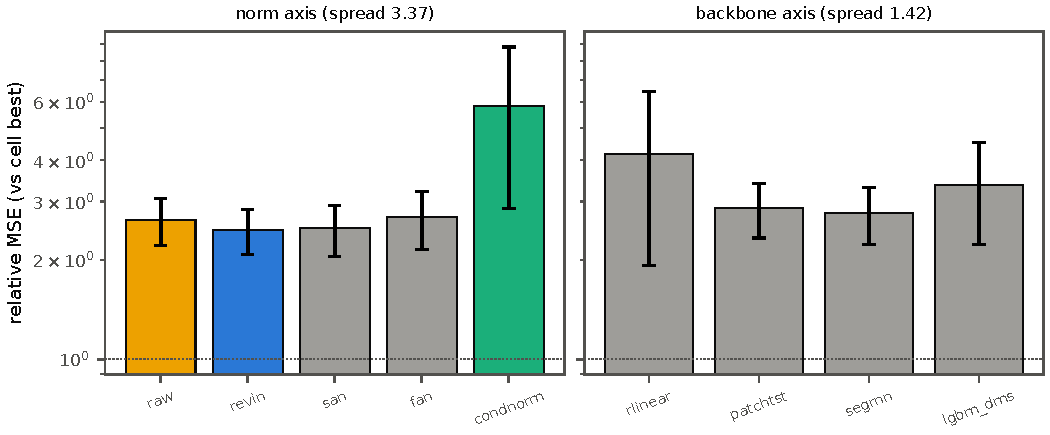
\includegraphics[width=.7\linewidth]{figures/fig4_factors.pdf}
\caption{Factor-level view of the variance attribution in \Cref{tab:attribution}: the normalization effect on error is almost entirely carried by its interaction with the dataset.}
\label{fig:factors}
\end{figure}

\Cref{tab:attribution} decomposes the variance of log test MSE over Block~A. Normalization-related terms account for $48.2\%$ of the variance, backbone-related terms for $0.6\%$. Strikingly, the normalization \emph{main} effect is tiny ($0.73\%$) while the normalization$\times$dataset interaction dominates ($47.12\%$): averaged over datasets, no normalization is better, because the \emph{sign} of the effect flips across datasets. That interaction is not a nuisance term---it \emph{is} the applicability boundary this paper characterizes (\Cref{fig:factors}). By contrast, which backbone sits under the normalization barely matters.

One decomposition of this decomposition is essential to reading it correctly, and we report it rather than leaving it to be found: the $47.12\%$ is carried by the single exogenous arm. Restricting the same computation to the four \emph{endogenous} arms \{\rawm, RevIN, SAN, FAN\}, the normalization$\times$dataset interaction falls to $0.43\%$ and all normalization-related terms total $0.73\%$, against $0.43\%$ for backbone-related terms. A reader could take this as deflating the headline; we take it as sharpening it. Within the endogenous family the choice of normalization is close to immaterial and no more consequential than the choice of backbone---which is consistent with the leaderboard literature, where these arms trade places across benchmarks without a stable winner. The variance that the normalization factor explains appears only when the family is widened to include an arm whose level statistics come from outside the target series. The boundary this paper characterizes therefore runs between endogenous and exogenous level handling, not between RevIN and its endogenous successors, and the attribution is best read as evidence for \emph{where} the boundary lies rather than as a claim that normalization is the dominant design axis in general.

\subsection{Horizon interaction}

\begin{figure}[t]
\centering
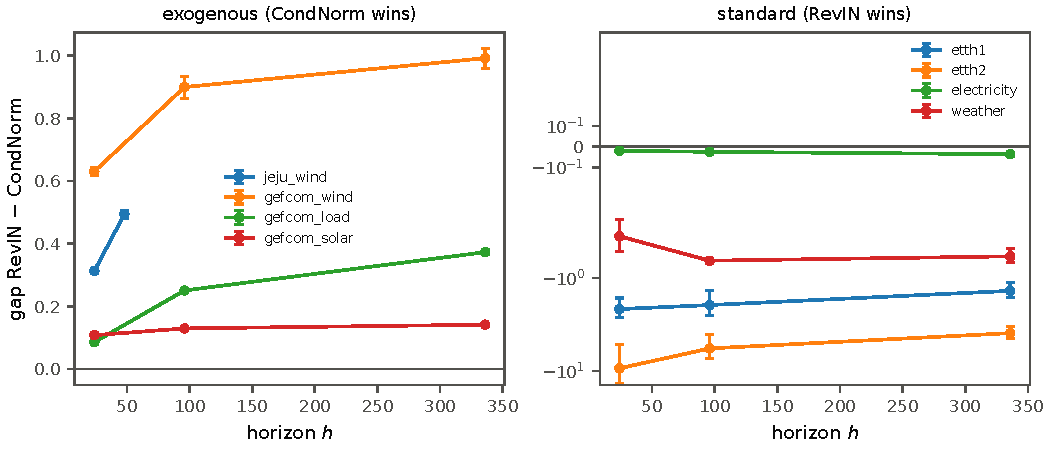
\includegraphics[width=.85\linewidth]{figures/fig5_horizon.pdf}
\caption{RevIN$-$CondNorm gap by horizon on the exogenously-driven group. The gap grows monotonically with $h$ on all four datasets, as predicted by \Cref{eq:prop3}.}
\label{fig:horizon}
\end{figure}

\Cref{sec:theory} predicts that the penalty of the frozen-statistics restoration rule grows with the horizon, since $\sx$ accumulates while the window statistics do not (\Cref{eq:prop3}). \Cref{fig:horizon} shows exactly this on real data: the RevIN$-$CondNorm gap increases monotonically in $h$ on all four exogenously-driven datasets. In particular, the Jeju Wind gap at $h=48$ exceeds that at $h=24$, an auxiliary prediction fixed in the pre-registration document. The horizon interaction confirmed on the synthetic grid (\Cref{sec:synthetic}) thus transfers to operational data.

\subsection{Robustness blocks}

\paragraph{Information parity (Block B)} Reported as the mechanism result in \Cref{sec:parity}; for completeness, within that block \cnm{} attains the lowest mean MSE for three of the five backbones (the linear mixer, the MLP mixer, and PatchTST-Cov) and is within $0.01$ of the best arm (\rawm$+$covariates) for LightGBM-Cov and SegRNN-Cov, so it is an adequate instrument but not the best method even here. By the Harvey-corrected DM test it is significantly better than RevIN in 11/11 exogenous cells for PatchTST-Cov, 10/11 for the linear and MLP mixers, 3/11 for LightGBM-Cov, and 2/11 for SegRNN-Cov. Full tables in \Cref{tab:covfair} (\Cref{app:ext}).

\paragraph{Published covariate architectures (Block C) and endogenous SOTA (Block D)} The pattern is not an artifact of our minimal covariate adapters. On the published covariate paths of TimeXer and iTransformer \citep{wang2024timexer,liu2024itransformer}---with built-in normalization removed and our five arms injected externally---the mean RevIN$-$CondNorm gap is $+0.4122$ for TimeXer-MS (55 pairs) and $+0.4282$ for iTransformer-MS, and CondNorm is best on all four exogenous datasets for both architectures (\Cref{tab:sota}, \Cref{app:ext}). Block~D, running the same architectures in their endogenous multivariate mode, reproduces the Block~A pattern qualitatively: CondNorm wins the exogenous group and loses the standard group.

\paragraph{Adaptive normalization and benchmark sanity} Two remaining objections fall to results already in \Cref{tab:main}. Against ``adaptive normalization already solves this'': SAN and FAN \citep{liu2023san,ye2024fan}, which learn non-stationary statistics rather than conditioning on covariates, lose to CondNorm on the \emph{entire} exogenous group---adapting the statistics endogenously is not a substitute for exogenous level information. Against ``the evaluation is biased toward energy data'': on the standard group our arms reproduce the literature's ranking and error levels (e.g., RevIN-family bests ETTh1 at $0.3771$), consistent with published results for these backbones \citep{li2023rlinear,qiu2024tfb}, and our conclusion there is precisely that instance normalization wins---the boundary, not either side of it, is the finding \citep{brigato2026champions}.
